% This document provides the style to be used for a MSc Thesis at the
% Parallel and Distributed Systems group
\documentclass[11pt,twoside,a4paper,openright]{report}

% use babel for proper hyphenation
\usepackage[british]{babel}
% Graphics: like the DUT logo on the front cover
\usepackage[dvips]{graphicx}
%Enables [H] for figures.
\usepackage{float}
% FONT: times
\usepackage{times}
% for url's use "\url{http://www.google.com/}"
\usepackage{url}

\begin{document}

%%%%%%%%%%%%%%%%%%%%%%%%%%%%%%%%%%%%%%%%%%%%%%%%%%%%%%%%%%%%%%%%%%%%%%%%%%%%%%%
\hoffset=1.63cm
\oddsidemargin=0in
\evensidemargin=0in
\textwidth=5in

%%%%%%%%%%%%%%%%%%%%%%%%%%%%%%%%%%%%%%%%%%%%%%%%%%%%%%%%%%%%%%%%%%%%%%%%%%%%%%%
\parindent=1em

\pagestyle{empty}

% FRONTCOVER
\begin{titlepage}

\null\vfill

\begin{center}
\LARGE{MultiChain:\\
       		An incremental step in a new distributed data structure}
\end{center}

\vspace{1.5cm}

\begin{center}
Steffan D. Norberhuis\\
steffan@norberhuis.nl
\end{center}

\vfill

\begin{figure}[!b]
\centering
\includegraphics[width={0.5\textwidth}]{pics/TUD_logo_color.eps}
\end{figure}

\vspace{2.0cm}

\end{titlepage}


% EMPTY PAGE
\cleardoublepage

\pagestyle{plain}

% TITLE PAGE: page i (hidden)
\include{titlepage}

% GRADUATION DATA AND ABSTRACT: pages ii and iii (hidden)
%De aankondiging bevat de spreker, titel, plaats, datum en tijd, samenstelling van de afstudeercommissie en een korte samenvatting (maximaal 25 regels).
\thispagestyle{empty}

\noindent \textbf{Author}\\
\begin{tabular}{l}
Steffan D. Norberhuis\\
\\
\end{tabular}\\
\noindent \textbf{Title}\\
\begin{tabular}{l}
MultiChain: an incremental step in a new distributed data structure\\
\\
\end{tabular}\\
\noindent \textbf{MSc presentation}\\
\begin{tabular}{l}
% <MM> DD, YYYY (like \today)
%TODO: #36 GRADUATION DATE\\
\\
\end{tabular}

\vspace{1.1cm}

\noindent \textbf{Graduation Committee}\\
\begin{tabular}{ll}
%TODO: #37 GRADUATION COMMITTEE & Delft University of Technology \\
% The order of listing the names: Graduation prof, supervisor(s), others ordered by title + alphabetical
%examples:
%prof. dr. ir. H. J. Sips (chair) & Delft University of Technology \\
%ir. dr. D. H. J. Epema           & Delft University of Technology \\
Prof. dr. ir. H. J. Sips            & Delft University Of Technology \\
dr. ir. J. A. Pouwelse        & Delft University of Technology \\
dr. ir. Z. Erkin              & Delft University of Technology \\
\end{tabular}

\begin{abstract} %de abstract bevat alleen een korte samenvatting van de inhoud van het onderzoek
Peer-to-peer networks are often large, collaborative networks where peers can join openly.
In these networks peers help other peers often in singular interactions and without direct reciprocity.
Peers can abuse and freeride.
The network without measures can fall into a tragedy of the commons
where no one helps another and only takes advantage of the generousity of peers.
Only if the reputation of a peer is publicly available at scale and tamper proof can a peer-to-peer network
escape the problems of freeriding and attain high utility for all participants.

This thesis focuses on creating the first step for a tamper proof reputation system within Tribler.
Tribler is a peer-to-peer BitTorrent system developed at the Delft University of Technology.
This first step, made by this thesis, is to design and implement a proof-of-concept bookkeeping system MultiChain.
MultiChain tracks the upload and download amounts of peers to eliminate free riding.
This bookkeeping system has to be scalable to be able to process enough transactions.

A new design of a distributed data structure that can be used as a ledger is introduced by this thesis.
This first step with MultiChain is already more resiliant to tampering than previous work.
The design of MultiChain is to have a chain of blocks for every peer.
A block contains a transaction shared between a peer.
This makes both chains of the peers intertwined and entangled between peers.
Abandoning a global ledger leads to a scalable data structure.
The implementation of the design is tested and experimented with within this thesis to validate it to correctly work.
Furthermore, a number of weak points are discussed that are future steps in creating a tamper proof reputation system.

\end{abstract}

\clearpage



\pagenumbering{roman}
\setcounter{page}{4}

% EMPTY PAGE: page iv
\cleardoublepage

% OPTIONAL QUOTATION: page v
%\include{quotation}
% EMPTY PAGE: page vi
%\cleardoublepage

% PREFACE: page v
\chapter*{Preface}
\addcontentsline{toc}{chapter}{Preface}
The huge increase in Bitcoin adoption, 
due to the increase in uncertainty in the security of traditional currency 
after the financial crisis in 2008, 
is only rivaled by the speculation of the enormous possibilities 
of the underlying technology of the blockchain.
The blockchain is the first technology, seen with real world adoption,
that allows to register transactions without a trusted third party.
But the blockchain has several limitations in scalabillity 
that will limit Bitcoins in fully replacing traditional currencies with a digital currency.
It also limits blockchain as a scalable basis for a large scale reputation system, 
similair to a digital currency, with vast amounts of transactions.
This motivated to research the properties and possibilities of a variant of the blockchain:
multichain.

\vspace{1\baselineskip}

\noindent
I would like to acknowledge several people that helped me during my master thesis.
First I would to heartly thank dr.ir. Johan Pouwelse for his mentoring and helping me in setting goals and achieving these goals in a timely manner.
Furthermore I would like to thank dr.ir. Cor-Paul Bezemer for his guidance and help with implementing within Tribler. 
I also would like to thank Elric Milon and Lipu Fei for answering countless questions and problems I encountered durng the programming phase of my thesis.
For the excellent feedback and help to improve my code I would like to thank dr.ir. Niels Zeilemaker.
I am also very thankful for the companionship I felt within my work room 
and I would like to thank especially Hans Bogerts BSc, Niels Doekeijmeier BSc and Ernst van der Hoeven BSc.
You certainly made my work more enjoyable.
Lastly I want to thank the trainers at the Sports and Culture Centre of the Delft University of Technology for giving an challenging outlet outside of my master thesis.

\vspace{1\baselineskip}

\noindent
Steffan Derk Norberhuis

\vspace{1\baselineskip}

\noindent
Delft, The Netherlands

\noindent
\today

% EMPTY PAGE: page vi
\cleardoublepage

% TABLE OF CONTENTS: starting at page vii
\tableofcontents

\cleardoublepage

\pagenumbering{arabic}
\setcounter{page}{1}

% INTRODUCTION: page 1
\chapter{Introduction}
\label{chp:introduction}
Tribler is a peer-to-peer file sharing program developed by the Delft University of Technology for research purposes.
Tribler expands the BitTorrent protocol and has added multiple improvements on this protocol.
The main focus of Tribler is to make security and privacy the default for Internet users and impossible to shutdown.
A fully distributed program, not relying on any central component, is needed to achieve this.
Tribler has been designed and build using this methodology\cite{Pouwelse-tribler}\cite{Bakker-tribler}.
This master thesis was conducted as part of the research mission to improve Tribler.

\vspace{1\baselineskip}

\noindent
TODO ORGANISATIONAL DESCRIPTION OF THESIS


%Problem description
\chapter{Problem Description}

The current Bitcoin protocol is depended on the block chain. 
Using a block chain limits Bitcoin in several ways.
These limitations on Bitcoin can be seen as the initial motivation 
for our work to improve the block chain.
But block chain and our improvement can be used in several other fields as well.

Bitcoin and how it uses the block chain technology will be introduced first.
After that the limitations imposed by the block chain will be explained.
Finally an overview will be given of how block chains and our improvements can be used in other fields.

\section{Bitcoin}
The core of the Bitcoin protocol is the block chain.
The block chain contains every transaction of bitcoins.

A transaction consists of three parts.
The public key of the new owner of the bitcoin,
the hash of combination of the previous transaction together with the public key of the new owner,
and the signature of the hash of the current owner.
The previous transaction is a transaction of the same bitcoin.
The ownership of the bitcoin by the current owner can be verified
by verifying the whole history of the bitcoin.
A transaction is usually shortend to Tx in Bitcoin related work and is used in images in this report.

\begin{figure}[H]
	\centerline{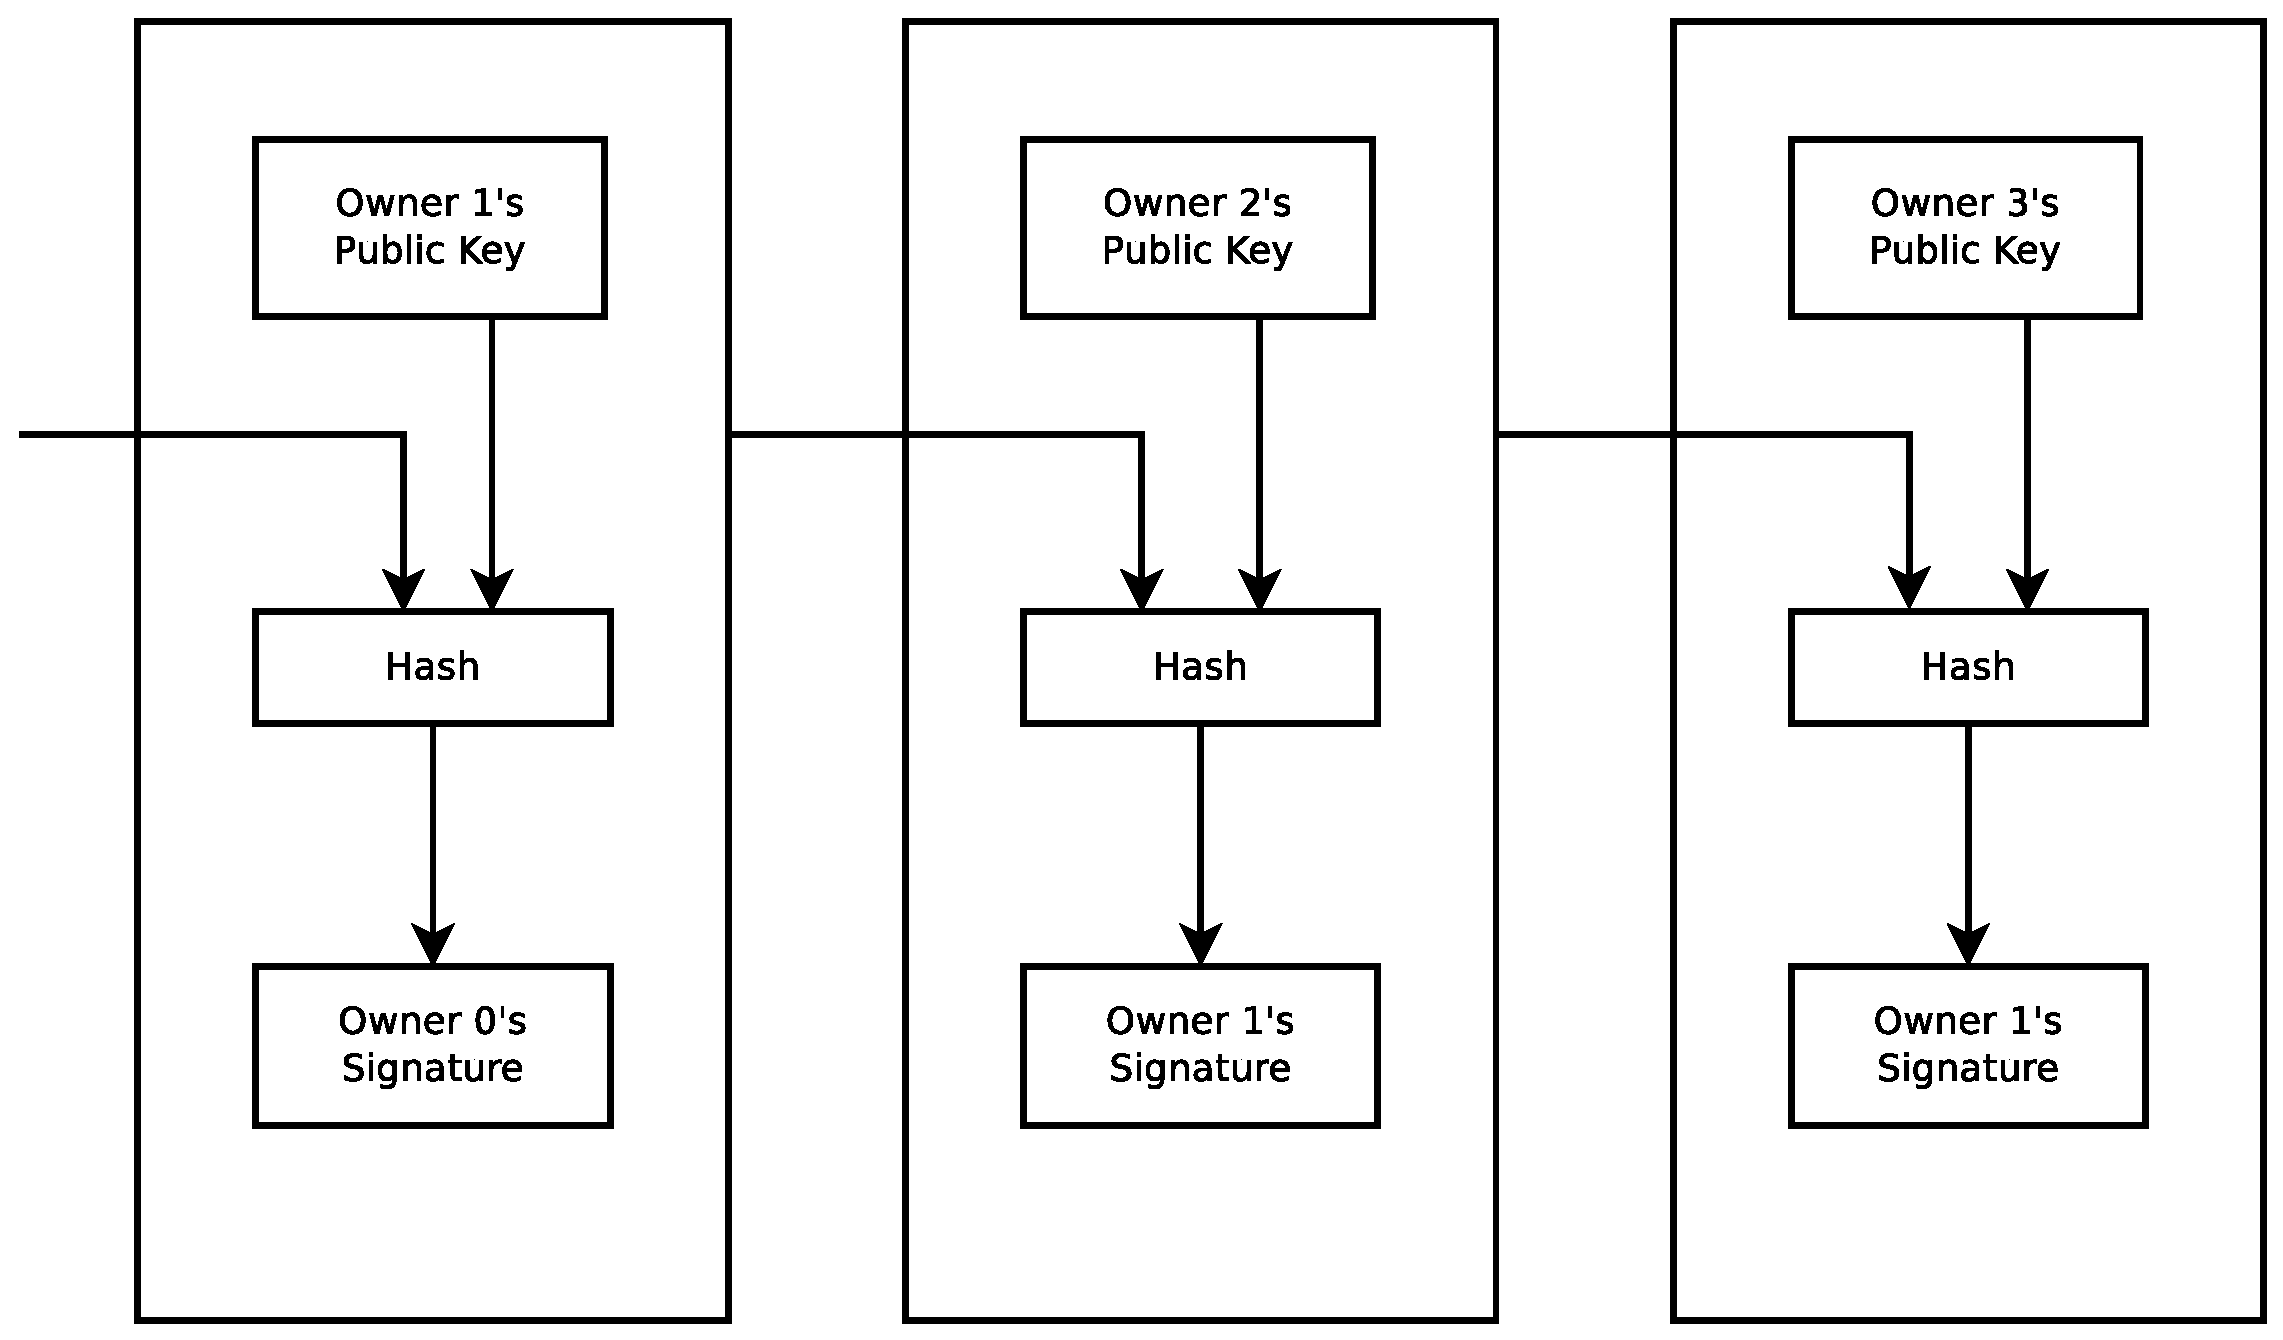
\includegraphics[scale=0.3]{problemDescription/figs/transactions.eps}}
	\caption{Transaction chain}
\end{figure}

Multiple transactions are aggregrated into a single block.
The next block is chained to the previous block by adding the hash of the previous block.
These blocks are created by nodes in the network, so called miners.
A miner receives transactions from other nodes in the Bitcoin network.
But the transactions are received in a non deterministic way induced by network characteristics.
The non deterministic nature causes blocks to differ from miner to miner.
The order of transactions has to be agreed upon by the network to eliminate this inconsistentcy.

Bitcoin uses election based upon Proof-Of-Work system.
To every block a nonce is added. 
This nonce is just a number that can be varied,
but is only sound if the result of the hash of the whole block starts with a certain number of zeros.
The amount of zeros required will be discussed later.


% CHAPTERS ... For instance: History/Prior Work, Design/Implementation, Experiments





% CONCLUSIONS AND FUTURE WORK

% BIBLIOGRAPHY
\bibliographystyle{bib/latex8}
\bibliography{bib/bibliography}

%\appendix

%\include{appendix_a}

\end{document}

